\section{Auswertung}
\subsection{Wheatstonesche Brücke}
Die gemessenen Werte für die Widerstände $ R_2, \: R_3 \: \text{und} \: R_4 $ zur
Bestimmung des unbekannten Widerstands $\text{R}_{x10} $ (Wert 10) befinden sich in
der untenstehenden Tabelle \ref{tab:tabe1}.
\begin{table}[H]
  \centering
  \caption{Messwerte der Wärmepumpe}
  \label{tab:tabe1}
    \begin{tabular}{S S S S S S}
    \toprule
    $ t  \: / \si{\second} $ & $ p_a \: / \si{\bar} $ & $ p_b \: / \si{\bar} $ &
    $ T_1 \: / \si{\kelvin} $ & $ T_2 \: / \si{\kelvin} $ & $ P \: / \: \si{\watt} $\\
    \midrule
    0 & 5.0 & 5.0 & 293.65 & 293.65 & 0 \\
    60 & 4.7 & 6.0 & 294.15 & 293.55 & 115 \\
    120 & 4.4 & 6.4 & 295.15 & 293.15 & 118 \\
    180 & 4.5 & 6.9 & 296.35 & 291.95 & 122 \\
    240 & 4.6 & 7.0 & 297.55 & 290.95 & 125 \\
    300 & 4.6 & 7.0 & 298.85 & 289.95 & 125 \\
    360 & 4.5 & 7.2 & 300.05 & 289.15 & 123 \\
    420 & 4.4 & 7.4 & 301.15 & 288.45 & 123 \\
    480 & 4.3 & 7.8 & 302.35 & 287.65 & 122 \\
    540 & 4.2 & 8.0 & 303.55 & 286.95 & 122 \\
    600 & 4.2 & 8.1 & 304.65 & 286.25 & 121 \\
    660 & 4.1 & 8.3 & 305.75 & 285.55 & 121 \\
    720 & 4.0 & 8.5 & 306.75 & 284.95 & 121 \\
    780 & 4.0 & 8.8 & 307.75 & 284.35 & 121 \\
    840 & 3.9 & 9.0 & 308.75 & 283.75 & 121 \\
    900 & 3.8 & 9.1 & 309.65 & 283.15 & 121 \\
    960 & 3.8 & 9.2 & 310.55 & 282.55 & 122 \\
    1020 & 3.8 & 9.5 & 311.45 & 282.05 & 122 \\
    1080 & 3.7 & 9.8 & 312.25 & 281.55 & 122 \\
    1140 & 3.7 & 10.0 & 313.05 & 281.15 & 122 \\
    1200 & 3.7 & 10.0 & 313.9 & 280.65 & 122 \\
    1260 & 3.6 & 10.2 & 314.65 & 280.25 & 123 \\
    1320 & 3.6 & 10.3 & 315.35 & 279.85 & 123 \\
    1380 & 3.6 & 10.6 & 316.15 & 279.45 & 124 \\
    1440 & 3.6 & 10.8 & 316.85 & 279.15 & 124 \\
    1500 & 3.6 & 11.0 & 317.55 & 278.75 & 124 \\
    1560 & 3.6 & 11.1 & 318.25 & 278.55 & 124 \\
    1620 & 3.6 & 11.2 & 318.95 & 278.25 & 125 \\
    1680 & 3.5 & 11.4 & 319.55 & 277.95 & 125 \\
    1740 & 3.5 & 11.5 & 320.15 & 277.65 & 125 \\
    1800 & 3.5 & 11.7 & 320.75 & 277.45 & 125 \\
    1860 & 3.5 & 11.9 & 321.35 & 277.25 & 125 \\
    1920 & 3.5 & 12.0 & 321.95 & 277.05 & 125 \\
    1980 & 3.5 & 12.1 & 322.45 & 276.95 & 125 \\








      \bottomrule
    \end{tabular}
\end{table}

\noindent Durch die Gleichung \ref{eqn:rx}
und Mittelung mit
\begin{equation}
  \bar{x} = \frac{1}{N} \sum_{i=1}^{N} x_i \: \: ,
\end{equation}
\noindent wobei der dazugehörige Fehler sich durch
\begin{equation}
  \increment \bar{x} = \frac{1}{\sqrt{N}} \sqrt{ \frac{1}{N-1} \sum_{i=1}^N
  (x_i - \bar{x})^2}
  \label{eqn:mitf}
\end{equation}
\noindent berechnet, ergibt sich somit:
\begin{equation*}
  \text{R}_{x10} = \SI{238.90 (64)}{\ohm}
\end{equation*}
\noindent Da das Verhältniss von $ \frac{R_3}{R_4} $ laut Hersteller mit einem
Fehler von $ \pm 0.5 \% $  behaftet ist und $ \text{R}_2 $ bis auf
0,2\% genau ist, muss hier auch die Gaußsche
Fehlerfortpflanzung mit der Formel
\begin{equation}
  \increment f = \sqrt{ \sum_{i=1}^N \left( \frac{\partial f}{\partial x_i}\right)^2
  \cdot (\increment x_i)^2  }
  \label{eqn:gaus}
\end{equation}
\noindent beachtet werden, durch die sich für $ \text{R}_{x10} $ ein Fehler von $ \pm 1,29 \: \si{\ohm} $
ergibt, welcher deutlich größer als der Mittelwertfehler ist und somit der signifikante
Fehler. Somit ergibt sich insgesamt
\begin{equation*}
  \text{R}_{x10} = \SI{239.7 (13)}{\ohm}
\end{equation*}


\noindent Analog lässt sich der Wert 11 berechnen, dessen Messwerte sich in Tabelle
\ref{tab:tabe2} befinden.
\begin{table}[H]
  \centering
  \caption{Wertetabelle für $\alpha$ und $C_V$.}
  \label{tab:tab2}
    \begin{tabular}{S S S S S}
    \toprule
    $ T\: \text{in}\: \si{\K} $ & $ {\alpha \cdot 10^{-6} \: \text{in}\: \si {\per\K}} $ &
    $ C_V \: \text{in}\: \si{\J\per\K\mol} $\\
    \midrule %Cv, a *10-6, Cv
    %0 & 1 & 1\\
    88.60\pm0.24 & 9.56\pm0.06 & 14.17\pm8.13  \\ %&3.6 & 318.97\pm0.85\\
    93.81\pm0.24 & 10.10\pm0.06 & 17.58\pm10.03 \\ %& 4.7 & 440.90\pm1.11\\
    99.74\pm0.24 & 10.66\pm0.05 & 15.52\pm8.84 \\ %& 5.1 & 508.68\pm1.21\\
    104.74\pm0.24 & 11.07\pm0.05 & 18.44\pm10.52 \\ %& 4.6 & 481.79\pm1.09\\
    110.94\pm0.24 &  11.54\pm0.05 & 14.86\pm8.45 \\ %& 5.3 & 587.97\pm1.27\\
    115.96\pm0.24 & 11.89\pm0.05 & 18.49\pm10.52 \\ %& 4.6 & 533.41\pm1.10\\
    121.47\pm0.24 &  12.22\pm0.05 & 16.83\pm9.57 \\ %& 4.9 & 595.21\pm1.17\\
    126.99\pm0.24 & 12.53\pm0.04 & 16.79\pm9.54 \\ %& 4.9 & 622.29\pm1.18\\
    131.58\pm0.24 & 12.77\pm0.04 & 20.42\pm11.62 \\ %& 4.2 & 552.62\pm1.01\\
    136.65\pm0.24 & 13.02\pm0.04 & 18.40\pm10.47 \\ %& 4.6 & 628.57\pm1.11\\
    141.49\pm0.24 & 13.24\pm0.04 & 19.28\pm10.97 \\ %& 4.4 & 622.54\pm1.07\\
    146.34\pm0.24 & 13.44\pm0.04 & 19.24\pm10.95 \\ %& 4.4 & 643.88\pm1.07\\
    150.95\pm0.24 & 13.62\pm0.04 & 20.22\pm11.52 \\ %& 4.3 & 649.11\pm1.05\\
    155.34\pm0.24 & 13.79\pm0.04 & 21.31\pm12.14 \\ %& 4.1 & 636.88\pm0.98\\
    159.97\pm0.24 & 13.95\pm0.04 & 20.12\pm11.47 \\ %& 4.3 & 687.89\pm1.05\\
    164.62\pm0.24 & 14.10\pm0.04 & 20.18\pm11.51 \\ %& 4.3 & 707.87\pm1.06\\
    168.79\pm0.25 & 14.23\pm0.04 & 22.54\pm12.86 \\ %& 3.9 & 658.27\pm0.95\\
    173.45\pm0.25 &  14.37\pm0.04 & 20.08\pm11.46 \\ %& 4.3 & 745.84\pm1.06\\
    178.13\pm0.25 &  14.50\pm0.04 & 20.04\pm11.44 \\ %& 4.3 & 765.94\pm1.06\\
    182.56\pm0.25 &  14.62\pm0.04 & 21.11\pm12.06\\
    192.70\pm0.25 &  14.87\pm0.04 & 18.41\pm10.47\\
    200.15\pm0.25 &  15.04\pm0.04 & 25.19\pm14.28\\
    208.87\pm0.25 &  15.23\pm0.04 & 21.43\pm12.18\\
    217.12\pm0.25 &  15.38\pm0.04 & 22.65\pm12.88\\
    225.15\pm0.25 &  15.53\pm0.03 & 23.27\pm13.24\\
    232.70\pm0.25 &  15.70\pm0.03 & 24.75\pm14.08\\
    240.53\pm0.25 &  15.74\pm0.03 & 23.84\pm13.58\\
    248.39\pm0.25 &  15.89\pm0.03 & 23.74\pm13.53& \\
    256.01\pm0.25 &  15.97\pm0.03 & 24.46\pm13.94 \\
    263.41\pm0.26 &  16.01\pm0.03 & 25.22\pm14.38 \\
    271.08\pm0.26 &  16.18\pm0.03 & 24.26\pm13.86 \\
    278.52\pm0.26 &  16.27\pm0.03 & 25.03\pm14.29&\\
    285.98\pm0.26 &  16.35\pm0.03 & 24.92\pm14.25 \\
    293.21\pm0.26 &  16.42\pm0.03 & 25.74\pm14.72 \\
    300.98\pm0.26 &  16.50\pm0.03 & 23.87\pm13.68 \\
    308.51\pm0.26 &  16.57\pm0.03 & 24.63\pm14.12\\



      \bottomrule
    \end{tabular}
\end{table}

\noindent Hierdurch ergibt sich für Wert 11:
\begin{equation*}
  \text{R}_{x11} = \SI{487.0 (26)}{\ohm}
\end{equation*}
\noindent wobei wieder der Gauß-Fehler der größere und somit signifikante ist. Der Fehler
des Mittelwerts beträgt dabei $ \pm 0,12 \: \si{\ohm}$.

\subsection{Kapazitätsmessbrücke}
Im zweiten Teil sollen zwei unbekannte Kapazitäten und eine RC-Kombination
vermessen werden. Die gemessenen Werte der ersten Kapazität $ \text{C}_{x3} $ (Wert 3) befinden
sich in Tabelle \ref{tab:tabe3} und die der zweiten Kapazität $ \text{C}_{x1} $
(Wert 1) in der
darauf folgenden Tabelle \ref{tab:tabe4}
\begin{table}
  \centering
  \caption{Messwerte für den ersten Doppelspalt.}
   \begin{tabular}{S S| S S | S S}
    \toprule
    $x/\; \si{\mm}$& $A/\;\si{\nA}$ &
    $x/\; \si{\mm}$& $A/\;\si{\nA}$ &
    $x/\; \si{\mm}$& $A/\;\si{\nA}$ \\
    \midrule

    15.0& 4.6& 23.0& 25.0& 29.5& 6.0\\
    15.5& 4.2& 23.5& 30.0& 30.0& 5.3\\
    16.0& 4.0& 24.0& 35.0& 30.5& 4.9\\
    16.5& 4.0& 24.25& 36.0& 31.0& 4.7\\
    17.0& 4.4& 24.5& 37.0& 31.5& 4.4\\
    17.5& 5.5& 24.75& 38.0& 32.0& 4.2\\
    18.0& 6.6& 25.00& 37.0& 32.5& 3.8\\
    18.5& 7.7& 25.25& 36.0& 33.0& 3.6\\
    19.0& 8.2& 25.5& 36.0& 33.5& 3.2\\
    19.5& 8.4& 26.0& 33.0& 34.0& 3.2\\
    20.0& 8.4& 26.5& 28.5& 34.5& 3.2\\
    20.25& 8.4& 27.0& 23.0& 35.0& 3.3\\
    20.5& 8,7& 27.5& 18.0& 35.5& 3.4\\
    21.0& 9.8& 28.0& 13.5& 36.0& 3.5\\
    21.5& 12.0& 28.5& 10.0\\
    22.0& 15.0& 29.0& 7.8\\
    22.5& 20.0& 29.25& 6.7\\


   \bottomrule
  \end{tabular}
  \label{tab:tabelle3}
\end{table}

\begin{table}[H]
  \centering
   \begin{tabular}{c c c c}
    \toprule
    Nummer der Oberwelle & $ U_{\text Theorie,Rechteck}\: / \si{\volt} $ &
    $ U_{\text Theorie,Dreick}\: / \si{\volt} $ & $ U_{\text Theorie,Sägezahn}\: / \si{\volt} $ \\
    \midrule
    1 & 1145 & 182 & 573 \\
    2 & 0 & 0 & 286 \\
    3 & 573 & 20 & 191 \\
    4 & 0 & 0 & 143 \\
    5 & 229 & 7 & 115 \\
    6 & 0 & 0 & 96 \\
    7 & 164 & 4 & 82 \\
    8 & 0 & 0 & 72 \\
    9 & 127 & 2 & 64 \\
    10 & 0 & 0 & 57 \\
    \bottomrule
  \end{tabular}
  \caption{Eingestellte Schwingungsamplituden.}
  \label{tab:tabe4}
\end{table}

\noindent Aus Gleichung \ref{eqn:cx}
ergibt sich damit für
\begin{align*}
  \text{C}_{x3} &= \SI{420.6 (29)}{\nano\farad} \\
  \text{C}_{x1} &= \SI{655.4 (35)}{\nano\farad}
\end{align*}
\noindent wobei bei $ \text{C}_{x3} $ der Fehler des Mittelwerts der größere war und bei
$ \text{C}_{x1} $ der Gauß-Fehler durch die Ungenauigkeit von $C_2$ mit $ \pm 0.2
\% $ und von dem Verhältniss von $ \frac{R_3}{R_4} $ mit $ \pm 0.5 \% $.
Der Gauß-Fehler von $ \text{C}_{x3} $ beträgt
dabei $ \pm 2,3 \: \si{\nano\farad} $ und der Mittelwertfehler von $ \text{C}_{x1} $
beträgt $ \pm 2,9 \: \si{\nano\farad} $.


\noindent Die RC-Kombination (Wert 9) mit der Kapazität $ \text{C}_{x9} $ und dem
Widerstand $ \text{R}_{x9} $ ergibt sich
mit den Werten aus Tabelle \ref{tab:tabe5} zu
\begin{align*}
  \text{C}_{x9} &= \SI{417 (13)}{\nano\farad} \\
  \text{R}_{x9} &= \SI{475 (14)}{\ohm}
\end{align*}
\noindent Dabei wurde für die Kapazität $ \text{C}_{x9} $ der Mittelwertfehler verwendet und
für den Widerstand $ \text{R}_{x9} $ der Fehler nach Gauß mit der Formel \ref{eqn:gaus}
, welcher durch die Abweichung des variablen Widerstands $R_2$ mit $ \pm 3 \% $
recht groß ausfällt. Der entsprechende Mittelwertfehler von $ \text{R}_{x9} $
beträgt dabei $ \pm 0,54 \: \si{\ohm} $ und der Gauß-Fehler von $ \text{C}_{x9} $ beträgt
$ \pm 2,56 \: \si{\nano\farad} $.
\begin{table}[H]
  \centering
  \caption{Bohrung 1 und 2, Vergleich der Sonden mit 1\;MHz und 2\;MHz.}
  \label{tab:tab5}
    \begin{tabular}{c c c c}
    \toprule
    Bohrung & $S_{\text{2\;MHz}}$/\;mm & $S_{\text{ 1\;MHz}}$/\;mm\\
    \midrule
    1 & 1,82 & 2,12\\
    2 & 1,83 & 1,97\\
    \bottomrule
    \end{tabular}
  \end{table}


\subsection{Induktivitätsmessbrücke}

Die Werte der unbekannten Induktivität $ \text{L}_{x16} $ und dem dazugehörigen
Widerstand $ \text{R}_{x16} $(Wert 16) sind in Tabelle
\ref{tab:tabe6} abzulesen.
\begin{table}[H]
  \centering
  \caption{Werte der Anpassungsschicht}
  \label{tab:tabe6}
    \begin{tabular}{S S S }
    \toprule
    $ \text{Zylinder} $ & $ \increment t [\mu\text{s}] $ &
    $ l_a \text{[mm]}$\\
    \midrule
    1 & 0.54 & 0.81 \\
    2 & 0.40 & 0.59 \\
    3 & 0.76 & 1.12 \\
    \text{1+2} & 0.49 & 0.73 \\
    4 & 0.70 & 1.03 \\
    \text{1+3} & 0.90 & 1.33 \\
    5 & 1.25 & 1.85 \\
    \text{1+4} & 0.69 & 1.02 \\
    6 & 0.44 & 0.66 \\

          \bottomrule
    \end{tabular}
  \end{table}

\noindent Durch die Gleichungen \ref{eqn:lx}
ergibt sich somit
\begin{align*}
  \text{R}_{x16} &= \SI{393 (12)}{\ohm} \\
  \text{L}_{x16} &= \SI{51.3 (21)}{\milli\henry}
\end{align*}
\noindent mit den Fehlern aus Gleichung \ref{eqn:gaus}, da die Mittelwertfehler aus Gleichung
\ref{eqn:mitf} mit
$ \pm 3,8 \: \si{\ohm} $ für $ \text{R}_{x16} $ und $ \pm 0,076 \: \si{\milli\henry} $
für $ \text{L}_{x16} $ jeweils kleiner sind.

\subsection{Maxwell-Brücke}

Bei der Messung wird eine Kapaziät $ \text{C}_{2} = \SI{450.0(9)}{\nano\farad} $
verwendet. Die Messwerte befinden sich in Tabelle \ref{tab:tabe7}
\begin{table}[H]
  \centering
  \caption{Parameter der gefitteten Gaußkurven}
  \label{tab:tabe7}
    \begin{tabular}{l l l l}
    \toprule
    $ a $ & $ b $ & $ c $
    & $ z \:/ \:\si{\kilo\electronvolt} $ \\
    \midrule
    593 \pm 23 & 1156 \pm 143 & 0.573 \pm 0.083 & 77.124 \pm 0.058 \\
    556 \pm 17 & 769 \pm 104 & 0.603 \pm 0.095 & 92.632 \pm 0.066 \\
    375.6 \pm 4.9 & 1335 \pm 25 & 0.772 \pm 0.017 & 186.090 \pm 0.012 \\
    252.8 \pm 6.2 & 1308 \pm 33 & 0.719 \pm 0.022 & 242.066 \pm 0.015 \\
    179.7 \pm 2.7 & 2711 \pm 14 & 0.7850 \pm 0.0048 & 295.3181 \pm 0.0033 \\
    130.2 \pm 4.2 & 4164 \pm 21 & 0.8586 \pm 0.0050 & 352.0054 \pm 0.0034 \\
    46.7 \pm 3.0 & 2230 \pm 12 & 1.1737 \pm 0.0076 & 609.2939 \pm 0.0052 \\
    31.3 \pm 1.1 & 64.9 \pm 4.2 & 1.33 \pm 0.10 & 665.409 \pm 0.070 \\
    31.3 \pm 1.3 & 158.5 \pm 4.6 & 1.451 \pm 0.051 & 768.246 \pm 0.034 \\
    30.9 \pm 1.0 & 38.9 \pm 3.9 & 1.29 \pm 0.16 & 785.87 \pm 0.10 \\
    30.7 \pm 1.0 & 46.6 \pm 4.1 & 1.20 \pm 0.13 & 806.244 \pm 0.085 \\
    26.3 \pm 1.1 & 72.9 \pm 3.7 & 1.68 \pm 0.10 & 934.015 \pm 0.067 \\
    18.2 \pm 1.9 & 292.3 \pm 5.8 & 1.782 \pm 0.043 & 1120.275 \pm 0.028 \\
    16.44 \pm 0.76 & 32.8 \pm 2.3 & 1.87 \pm 0.16  & 1155.44 \pm 0.10 \\
    13.1 \pm 1.1 & 98.2 \pm 3.1 & 2.037 \pm 0.078 & 1238.098 \pm 0.051 \\
    16.17 \pm 0.93 & 55.9 \pm 2.7 & 1.91 \pm 0.11 & 1377.862 \pm 0.074 \\
    17.5 \pm 1.3 & 25.6 \pm 3.8 & 1.95 \pm 0.36 & 1408.31 \pm 0.23 \\
    13.89 \pm 0.95 & 19.6 \pm 2.4 & 2.33 \pm 0.36 & 1509.44 \pm 0.22 \\
    4.78 \pm 0.63 & 12.2 \pm 1.3 & 2.96 \pm 0.40 & 1661.07 \pm 0.24 \\
    3.029 \pm 0.73 & 28.2 \pm 1.6 & 2.75 \pm 0.20 & 1729.76 \pm 0.12 \\
    3.0 \pm 1.79 & 145.9 \pm 3.9 & 2.725 \pm 0.093 & 1764.689 \pm 0.057 \\
    3.56 \pm 0.78 & 20.2 \pm 1.7 & 2.77 \pm 0.29 & 1847.40 \pm 0.18 \\
    0.71 \pm 0.87 & 29.1 \pm 1.6 & 3.35 \pm 0.24 & 2204.71 \pm 0.13 \\



          \bottomrule

    \end{tabular}
\end{table}

\noindent Aus den Gleichungen \ref{eqn:mx}
ergibt sich\begin{align*}
  \text{R}_{x16} &= \SI{330 (29)}{\ohm} \\
  \text{L}_{x16} &= \SI{49 (14)}{\milli\henry}
\end{align*}
\noindent wobei der Mittelwertfehler für $ \text{R}_{x16} $ verwendet wurde (Gauß-Fehler =
$ \pm 14 \: \si{\ohm} $) und der Gauß-Fehler für $ \text{L}_{x16} $ (Mittelwertfehler=
$ \pm 4,4 \: \si{\milli\henry} $).

\subsection{Wien-Robinson-Brücke}
Die Messung der Wien-Robinson-Brücke wird mit einer Kapazität C=$ 992 \: \si{\nano\farad}$
und einem Widerstand von R= $664\: \si{\ohm}$ durchgeführt. Die Messwerte sind in Tabelle
\ref{tab:tabe8} dargestellt.

\begin{table}[H]
  \centering
  \caption{Werte der Messreihe die Wien-Robinson-brücke}
  \label{tab:tabe8}
    \begin{tabular}{c c c c}
    \toprule
    $ \nu \: / \: \si{\hertz} $ & $\text{U}_b \: / \: \si{\volt} $ &
    $\text{U}_s \: / \: \si{\volt} $ &
    $\frac{U_b}{U_s}$ \\
    \midrule
    20 & 0.120 & 3.08 & 0.039 \\
    50 & 0.248 & 4.56 & 0.054 \\
    100 & 0.320 & 4.64 & 0.069 \\
    150 & 0.264 & 4.56 & 0.058 \\
    200 & 0.136 & 4.50 & 0.030 \\
    220 & 0.072 & 4.48 & 0.016 \\
    230 & 0.032 & 4.48 & 0.007 \\
    240 & 0.024 & 4.48 & 0.005 \\
    242 & 0.016 & 4.48 & 0.004 \\
    250 & 0.040 & 4.48 & 0.009 \\
    265 & 0.080 & 4.48 & 0.018 \\
    300 & 0.298 & 4.56 & 0.065 \\
    500 & 0.704 & 4.56 & 0.154 \\
    1000 & 1.17 & 4.32 & 0.271 \\
    3000 & 1.41 & 4.28 & 0.330 \\
    10000 & 1.44 & 4.24 & 0.340 \\
    20000 & 1.44 & 4.24 & 0.340 \\
    30000 & 1.44 & 4.24 & 0.340 \\

    \bottomrule
    \end{tabular}
\end{table}


\noindent In Abbildung \ref{fig:plot} ist das Verhältniss $\frac{U_b}{U_s}$ gegen
$\frac{\nu}{\nu_0} $ aufgetragen.

\begin{figure}[H]
  \centering
  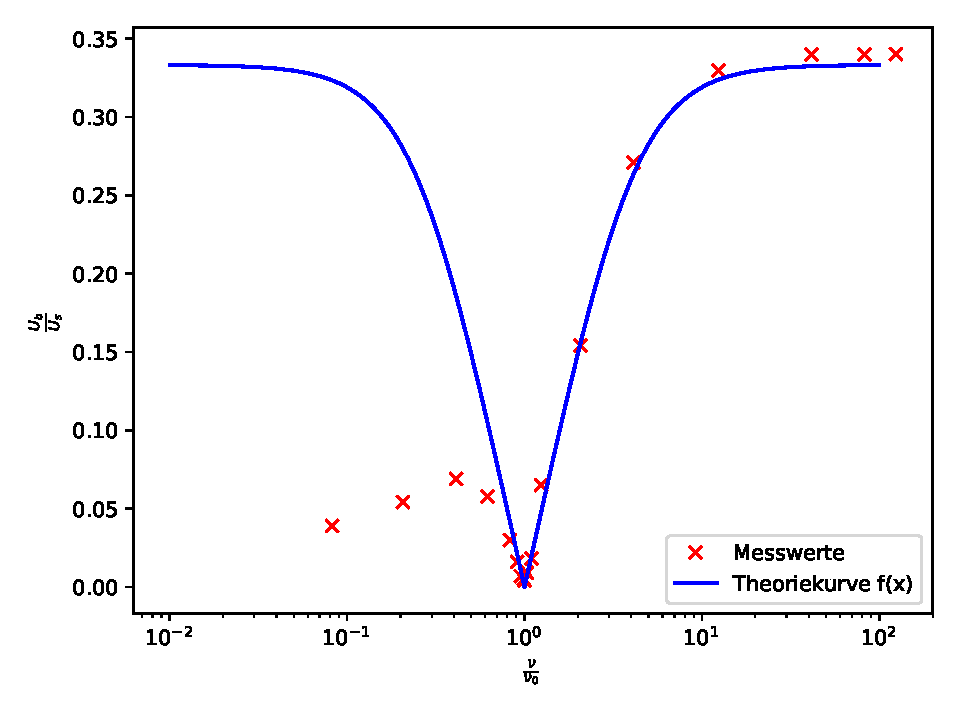
\includegraphics{plot.pdf}
  \caption{Diagramm zur Wien-Robinson-Brücke}
  \label{fig:plot}
\end{figure}

\noindent Der Theoriwert für $\omega_0$ ergibt sich zu
\begin{equation*}
  \omega_0 = \frac{1}{RC} = 1518,17 \: \si{\hertz}
\end{equation*}
\noindent und somit
\begin{equation*}
  \nu_0 = \frac{\omega_0}{2\pi} = 241,62 \: \si{\hertz}
\end{equation*}

\subsection{Klirrfaktorbestimmung}

Das Minimum der Frequenz liegt bei einer Frequenz von 242 $\si{\hertz}$
mit einer Brückenspannung $\text{U}_b = 0,016 \: \si{\volt} \: \text{und} \:
\text{U}_s = 4,48 \: \si{\volt} $.
Durch die Gleichung \ref{eqn:betrag}
ergibt sich f(2) zu
\begin{equation*}
  f(\Omega =2) \approx 0.14907
\end{equation*}
\noindent Daraus folgt, dass
\begin{equation*}
  \text{U}_2 = \frac{\text{U}_b}{f(2)} = \SI{0.107}{\volt}
\end{equation*}
\noindent und schlussendlich
\begin{equation*}
  \text{k}= \frac{\text{U}_2}{\text{U}_1} = 0.024
\end{equation*}
